\section{Results}
\label{sec:results}

\subsection{Effect of the Split Protocol (RQ1)}
\label{sec:leak}
Table~\ref{tab:leak} evaluates the same 21 raw columns under three protocols. When every discomfort grade is oversampled to 5,243 samples before a 70/15/15 row split, an untuned gradient-boosting classifier reaches \LeakOldAcc\,\% accuracy, \LeakOldRecall\,\% recall, MCC \LeakOldMCC{} and ROC-AUC \LeakOldRocAuc; \LeakDupPos{} of the \LeakTestPos{} positive test rows (\LeakDupPct\,\%) have an exact duplicate in the training split, and every session contributes to both splits. Without oversampling, a row-level split still gives ROC-AUC \LeakRowRocAuc{} (accuracy \LeakRowAcc\,\%), because adjacent seconds of the same session are nearly identical and carry the same label. With a session-grouped split, the same classifier falls to ROC-AUC \LeakGrpRocAuc{} (MCC \LeakGrpMCC). The earlier E-DDQN implementation behaves the same way: \OrigOldRecall\,\% recall and MCC \OrigOldMCC{} on the oversampled row-level partition, but MCC \OrigGrpMCC{} on a grouped partition. Near-perfect scores on these data therefore measure the recognition of sessions seen during training, not the detection of cybersickness in new sessions, and they are obtained without any reinforcement learning. All results below use the leakage-free protocol of Section~\ref{sec:protocol}.

\begin{table*}[t]
\centering
\caption{Effect of the evaluation protocol on the same data (21 raw columns of the curated release; test-split metrics). ``Proxy'' marks the reconstruction of the earlier protocol, whose 41-feature input files were not available.}
\label{tab:leak}
\resizebox{\textwidth}{!}{\begin{tabular}{llccccc}
\toprule
Model & Evaluation protocol & Acc. & Recall & Spec. & MCC & ROC-AUC \\
\midrule
HGB & Oversample to 5,243/grade, then 70/15/15 row split (earlier protocol) & 97.6 & 99.8 & 91.0 & 0.935 & 0.995 \\
HGB & Row-level random split, no oversampling & 95.3 & 94.1 & 96.3 & 0.905 & 0.992 \\
HGB & Grouped 5-fold split (session-linkage groups) & 52.2 & 33.6 & 66.9 & 0.005 & 0.523 \\
E-DDQN (earlier code) & Earlier script, earlier protocol (proxy) & 95.2 & 99.2 & 83.1 & 0.870 & -- \\
E-DDQN (earlier code) & Earlier script, grouped split (proxy) & 41.1 & 92.1 & 7.7 & $-$0.004 & -- \\
\bottomrule
\end{tabular}
}
\end{table*}

\subsection{Leakage-Free Comparison under the 5:1 Cost (RQ3)}
\label{sec:main}
Table~\ref{tab:main} reports every model tuned, checkpointed and thresholded on validation groups only and scored once on the outer-test groups (all \nSamplesEval{} samples, \nSessionsEval{} sessions). Two facts dominate. First, the detection problem is hard once sessions and participants are not shared: among the primary models, the best ROC-AUC is \HGBCostRocAucMean{} (HGB) and \RFCostRocAucMean{} (random forest), against a prevalence of 0.44. Second, under a 5:1 cost the cost-minimizing operating point of every model lies close to ``always alarm'' (cost \AlwaysCost): validation-selected thresholds yield high recall but false-positive rates of \DOneFPRMin--\DOneFPRMax\,\%. The random forest has the lowest cost, both as a mean over seeds (\RFCostCostMean$\pm$\RFCostCostSD) and as a seed ensemble (\PHEnsRFCost).

E-DDQN ranks last of the \nModels{} primary models: recall \EDDQNCostRecallMean$\pm$\EDDQNCostRecallSD\,\%, specificity \EDDQNCostSpecMean$\pm$\EDDQNCostSpecSD\,\%, cost \EDDQNCostCostMean$\pm$\EDDQNCostCostSD{} (higher than always alarming), ROC-AUC \EDDQNCostRocAucMean$\pm$\EDDQNCostRocAucSD{} and MCC \EDDQNCostMCCMean; its seed ensemble is worse still (cost \PHEnsEDDQNCost, recall \PHEnsEDDQNRecall\,\%). The standard DQN reaches cost \DQNCostCostMean{} and ROC-AUC \DQNCostRocAucMean, and the contextual-bandit variant E-CB cost \ECBCostCostMean{} and ROC-AUC \ECBCostRocAucMean. E-DDQN therefore does not improve on the standard DQN in this controlled comparison.

\begin{table*}[t]
\centering
\caption{Leakage-free comparison (rule D1: threshold minimizing the 5:1 cost on pooled inner-validation predictions; \nSamplesEval{} outer-test samples; recall, specificity and balanced accuracy in \%). Left: mean~$\pm$~SD over five seeds. Right: the seed ensemble (mean score over the five seeds, thresholded on the mean inner-OOF score; Section~\ref{sec:seeds}), whose predictions are used for the paired tests, confidence intervals, comparison with always alarming and cost curves; FN and FP are exact counts. Bold: lowest cost among the primary models. HGB, logistic regression and the post-hoc baselines are deterministic given the data, hence SD = 0 and identical left and right values. Precision, F1, accuracy and G-mean: Supplementary Sec.~S3.1.}
\label{tab:main}
\resizebox{\textwidth}{!}{\begin{tabular}{lccccccc|ccccc}
\toprule
 & \multicolumn{7}{c|}{Mean $\pm$ SD over five seeds} & \multicolumn{5}{c}{Seed ensemble (paired tests)} \\
Model & Recall & Spec. & Bal.\ acc. & MCC & Cost$_{5:1}$ & ROC-AUC & PR-AUC & Recall & Spec. & Cost$_{5:1}$ & FN & FP \\
\midrule
\textbf{E-DDQN} & 93.4$\pm$2.5 & 7.4$\pm$2.7 & 50.4$\pm$1.2 & 0.016$\pm$0.054 & 0.663$\pm$0.048 & 0.538$\pm$0.016 & 0.483$\pm$0.019 & 90.4 & 8.1 & 0.726 & 400 & 4,820 \\
E-CB & 97.1$\pm$2.9 & 8.4$\pm$2.8 & 52.8$\pm$1.2 & 0.122$\pm$0.052 & 0.575$\pm$0.055 & 0.653$\pm$0.011 & 0.562$\pm$0.006 & 96.6 & 14.6 & 0.552 & 140 & 4,480 \\
DQN & 95.2$\pm$2.7 & 14.5$\pm$4.9 & 54.8$\pm$1.6 & 0.158$\pm$0.038 & 0.584$\pm$0.040 & 0.661$\pm$0.013 & 0.595$\pm$0.022 & 96.9 & 16.3 & 0.536 & 129 & 4,391 \\
CS-MLP & 99.4$\pm$0.7 & 2.8$\pm$1.9 & 51.1$\pm$0.8 & 0.072$\pm$0.049 & 0.557$\pm$0.012 & 0.644$\pm$0.018 & 0.521$\pm$0.022 & 99.4 & 6.1 & 0.537 & 23 & 4,925 \\
LogReg & 99.1$\pm$0.0 & 8.1$\pm$0.0 & 53.6$\pm$0.0 & 0.167$\pm$0.000 & 0.532$\pm$0.000 & 0.626$\pm$0.000 & 0.576$\pm$0.000 & 99.1 & 8.1 & 0.532 & 36 & 4,817 \\
HGB & 97.0$\pm$0.0 & 14.6$\pm$0.0 & 55.8$\pm$0.0 & 0.197$\pm$0.000 & 0.543$\pm$0.000 & 0.692$\pm$0.000 & 0.593$\pm$0.000 & 97.0 & 14.6 & 0.543 & 124 & 4,479 \\
RF & 98.5$\pm$0.3 & 18.2$\pm$0.7 & 58.3$\pm$0.3 & 0.266$\pm$0.004 & \textbf{0.491$\pm$0.003} & 0.688$\pm$0.002 & 0.548$\pm$0.001 & 98.7 & 18.3 & \textbf{0.485} & 54 & 4,281 \\
\midrule
\multicolumn{13}{l}{\emph{Post-hoc exposure-time baselines (added after the primary analysis)}} \\
Time-LR (elapsed time) & 96.7$\pm$0.0 & 15.0$\pm$0.0 & 55.8$\pm$0.0 & 0.194$\pm$0.000 & 0.548$\pm$0.000 & 0.704$\pm$0.000 & 0.605$\pm$0.000 & 96.7 & 15.0 & 0.548 & 138 & 4,457 \\
Time+game HGB & 97.4$\pm$0.0 & 17.6$\pm$0.0 & 57.5$\pm$0.0 & 0.239$\pm$0.000 & 0.517$\pm$0.000 & 0.676$\pm$0.000 & 0.550$\pm$0.000 & 97.4 & 17.6 & 0.517 & 107 & 4,319 \\
\midrule
Always alarm & 100.0 & 0.0 & 50.0 & 0.000 & 0.558 & -- & -- & 100.0 & 0.0 & 0.558 & 0 & 5,243 \\
Never alarm & 0.0 & 100.0 & 50.0 & 0.000 & 2.208 & -- & -- & 0.0 & 100.0 & 2.208 & 4,147 & 0 \\
\bottomrule
\end{tabular}
}
\end{table*}

\subsection{Exposure-Time Baselines}
\label{sec:time}
The post-hoc baselines (Table~\ref{tab:main}, Fig.~\ref{fig:roc}) show what the primary models have learned. Time-LR, a logistic regression on elapsed time alone, reaches ROC-AUC \PHTimeLRRocAucMean{} and PR-AUC \PHTimeLRPrAucMean, the highest values of all models. Its ROC-AUC does not differ significantly from that of the random forest (difference \PHTimeLRvsRFAuc, 95\,\% CI \PHTimeLRvsRFAucLow{} to \PHTimeLRvsRFAucHigh; group bootstrap); the interval is wide, so equivalence is not established either. At the 5:1 operating point, however, the random forest has a lower cost than Time-LR (seed ensembles \PHEnsRFCost{} vs.\ \PHEnsTimeLRCost; difference \PHTimeLRvsRFCost, CI \PHTimeLRvsRFCostLow{} to \PHTimeLRvsRFCostHigh, $p=$\,\PHTimeLRvsRFCostP), so the additional inputs help the forest at the operating point (fewer missed events and fewer false alarms in the seed ensemble; Table~\ref{tab:main}). Adding the game indicator (Time+game HGB) gives cost \PHTimeHGBCostMean{} and ROC-AUC \PHTimeHGBRocAucMean, again not significantly different from the random forest (cost difference \PHTimeHGBvsRFCost, $p=$\,\PHTimeHGBvsRFCostP; ROC-AUC difference \PHTimeHGBvsRFAuc, $p=$\,\PHTimeHGBvsRFAucP). Both minimal baselines rank seconds better than E-DDQN (seed-ensemble ROC-AUC difference for Time-LR \PHTimeLRvsEDDQNAuc, CI \PHTimeLRvsEDDQNAucLow{} to \PHTimeLRvsEDDQNAucHigh). On these data, therefore, no model was shown to discriminate better than a population onset curve, in which cybersickness becomes more likely the longer a session lasts; the wide intervals leave open modest gains that a sample of \nGroupsEval{} groups cannot detect.

\begin{figure}[t]
\centering
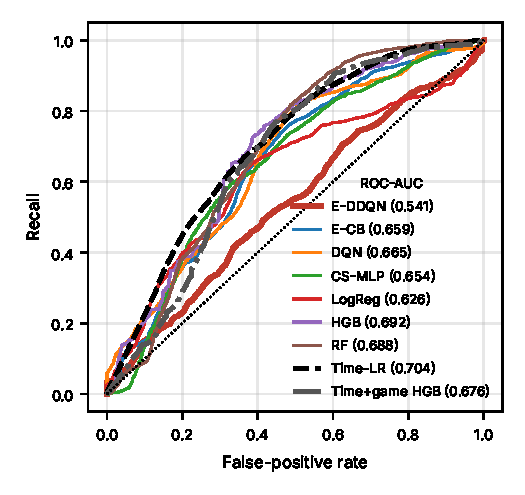
\includegraphics[width=\columnwidth]{figs/posthoc_roc.pdf}
\caption{ROC curves of the seed-ensemble scores, pooled over the five outer-test folds, for the seven primary models and the two post-hoc exposure-time baselines (dashed and dash-dotted). The legend gives the ROC-AUC of the seed-ensemble score, which can differ slightly from the seed means in Table~\ref{tab:main}.}
\label{fig:roc}
\end{figure}

\subsection{Operating Points, Cost Ratios and the Asymmetric Reward}
\label{sec:op}
Table~\ref{tab:ops} contrasts three operating rules. With the untuned Bayes cut-off $\hat p\ge 1/6$ (rule D0)---for the asymmetric agents this is the greedy policy $\arg\max_a Q(s,a)$---E-DDQN obtains recall \EDDQNBayesRecallMean\,\% at specificity \EDDQNBayesSpecMean\,\% (cost \EDDQNBayesCostMean), whereas the random forest obtains recall \RFBayesRecallMean\,\% at specificity \RFBayesSpecMean\,\% (cost \RFBayesCostMean). When every model is held to a validation recall of at least 0.95, the random forest again has the lowest cost (\RFRecCostMean; E-DDQN \EDDQNRecCostMean). At validation-matched recall targets (Table~\ref{tab:matched}), the thresholds transfer worst for E-DDQN: at both recall targets it attains lower test recall than every supervised model, and at the 0.95 target it also has a higher false-positive rate than all of them. Reading the ROC curves at fixed recall (descriptive only), the false-positive rate at 95\,\% recall is \EDDQNRocFPRatNineFive\,\% for E-DDQN and \RFRocFPRatNineFive\,\% for the random forest. Because the reward encodes the same 5:1 operating point as a cost-weighted classifier (Eq.~\eqref{eq:margin}), the asymmetric reward provides no advantage that cost-weighted training plus a validation-selected threshold does not already provide.

The cost curves of Fig.~\ref{fig:costcurves} show how much the choice of the 5:1 ratio matters. At ratios of 1.5--2, where the cost-optimal policy is not close to a trivial one, the relative costs of all models except E-DDQN lie between \PHCcLowRMin{} and \PHCcLowRMax{} (random forest: \PHCcRFTwo{} at $R=2$). As $R$ grows, every curve approaches 1, because the Bayes cut-off $1/(1+R)$ falls far below the prevalence and alarming almost always becomes optimal; at $R=5$ the random forest's relative cost is \PHCcRFFive. The random forest stays below the trivial policies at all \PHCcNratios{} ratios, E-DDQN at \PHCcEDDQNBelow{} of them. The negative safety result is therefore not an artifact of the particular ratio: the models discriminate weakly at every ratio, and the 5:1 ratio places the operating point where that weakness is most visible.

\begin{figure}[t]
\centering
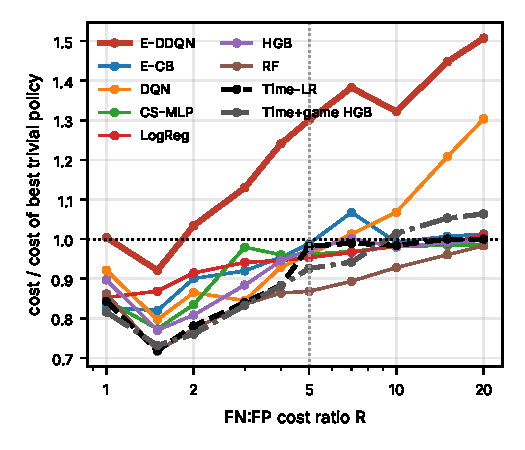
\includegraphics[width=\columnwidth]{figs/posthoc_cost_curves.pdf}
\caption{Validation-chosen cost curves (post hoc): for each false-negative to false-positive cost ratio $R$, the threshold minimizing $R\,\mathrm{FN}+\mathrm{FP}$ on the inner-validation predictions is applied to the outer-test fold; the pooled test cost of the seed ensemble is divided by the cost of the better trivial policy (always or never alarm). Values below 1 improve on the trivial policy; the dotted vertical line marks the 5:1 ratio.}
\label{fig:costcurves}
\end{figure}

\begin{table}[t]
\centering
\caption{Expected 5:1 cost (mean over seeds) under three operating rules chosen without test data.}
\label{tab:ops}
\footnotesize
\begin{tabular}{lccc}
\toprule
Model & D1: min cost & D0: $\hat p\ge 1/6$ & val.\ recall $\ge$ 0.95 \\
\midrule
E-DDQN & \EDDQNCostCostMean & \EDDQNBayesCostMean & \EDDQNRecCostMean \\
E-CB & \ECBCostCostMean & \ECBBayesCostMean & \ECBRecCostMean \\
DQN & \DQNCostCostMean & \DQNBayesCostMean & \DQNRecCostMean \\
CS-MLP & \CSMLPCostCostMean & \CSMLPBayesCostMean & \CSMLPRecCostMean \\
LogReg & \LRCostCostMean & \LRBayesCostMean & \LRRecCostMean \\
HGB & \HGBCostCostMean & \HGBBayesCostMean & \HGBRecCostMean \\
RF & \RFCostCostMean & \RFBayesCostMean & \RFRecCostMean \\
\midrule
Always alarm & \AlwaysCost & \AlwaysCost & \AlwaysCost \\
\bottomrule
\end{tabular}
\end{table}

\begin{table*}[t]
\centering
\caption{Matched operating points: thresholds chosen on validation predictions to reach the stated recall or specificity; test recall (\%), false-positive rate (\%) and false-positive count of the seed ensemble.}
\label{tab:matched}
\footnotesize
\begin{tabular}{lccccccccc}
\toprule
 & \multicolumn{3}{c}{val. recall $\ge$ 0.90} & \multicolumn{3}{c}{val. recall $\ge$ 0.95} & \multicolumn{3}{c}{val. specificity $\ge$ 0.80} \\
Model & Rec. & FPR & FP & Rec. & FPR & FP & Rec. & FPR & FP \\
\midrule
E-DDQN & 81.7 & 77.0 & 4,036 & 84.5 & 86.6 & 4,539 & 25.2 & 18.6 & 974 \\
E-CB & 88.6 & 68.0 & 3,565 & 92.4 & 78.1 & 4,093 & 31.2 & 17.4 & 910 \\
DQN & 88.0 & 64.2 & 3,366 & 91.7 & 72.7 & 3,810 & 32.2 & 14.2 & 743 \\
CS-MLP & 94.1 & 78.4 & 4,111 & 97.5 & 85.1 & 4,463 & 24.2 & 12.7 & 666 \\
LogReg & 92.8 & 73.5 & 3,856 & 97.2 & 81.7 & 4,285 & 37.7 & 22.5 & 1,181 \\
HGB & 95.4 & 72.2 & 3,785 & 97.5 & 81.7 & 4,282 & 24.3 & 11.3 & 594 \\
RF & 93.7 & 64.0 & 3,358 & 96.9 & 74.3 & 3,896 & 21.0 & 13.3 & 695 \\
\bottomrule
\end{tabular}

\end{table*}

\subsection{Statistical Comparison}
\label{sec:stats}
Table~\ref{tab:paired} compares E-DDQN with every other primary model on identical test samples (seed ensembles, rule D1). Sample-level McNemar tests give $p<0.001$ for every pair, but they treat \nSamplesEval{} strongly autocorrelated seconds as independent and overstate the evidence; they are reported for completeness, with the contingency identity $b-c=\mathrm{err}_B-\mathrm{err}_A$ checked and recomputed with an independent library. The primary inference is the group bootstrap, which resamples the \nGroupsEval{} independent units. E-DDQN's seed-ensemble cost (\PHEnsEDDQNCost) exceeds that of every other primary model by \PairDOneECBCostDiff{} to \PairDOneRFCostDiff. These ensemble differences are larger than the corresponding differences of seed means in Table~\ref{tab:main} (\PHMeanDiffDQN{} to \PHMeanDiffRF) because E-DDQN's ensemble is worse than its average seed (Section~\ref{sec:seeds}); after Holm adjustment over the six comparisons, only the difference from the random forest remains significant (\PairDOneRFCostDiff, 95\,\% CI \PairDOneRFCostLo{} to \PairDOneRFCostHi; adjusted $p=$\,\PHHolmRF), whereas the adjusted $p$-values for the other five comparisons lie between \PHHolmECB{} and \PHHolmHGB. In particular, the difference from the standard DQN (\PairDOneDQNCostDiff; seed means \PHMeanDiffDQN) is not significant (unadjusted $p=$\,\PairDOneDQNPboot).

These conclusions are robust to the choice of resampling unit and to individual groups. Resampling the \nSessionsEval{} sessions instead of the groups gives the same pattern (E-DDQN vs.\ random forest: CI \PHSesRFLow{} to \PHSesRFHigh, Holm-adjusted $p=$\,\PHSesRFHolm). In a leave-one-group-out jackknife over the \PHJkGroups{} groups, the cost difference between E-DDQN and the random forest ranges from \PHJkEDDQNvsRFMin{} to \PHJkEDDQNvsRFMax{} and never changes sign; the same holds for every other comparison with E-DDQN. Compared with always alarming, the random forest's seed-ensemble cost differs by \PHAlwRFGrp{} (CI \PHAlwRFGrpLow{} to \PHAlwRFGrpHigh; unadjusted $p=$\,\PHAlwRFGrpP), but after Holm adjustment over the nine models this is not significant ($p=$\,\PHAlwRFGrpHolm); E-DDQN's seed-ensemble cost differs from that of always alarming by \PHAlwEDDQNGrp{} (CI \PHAlwEDDQNGrpLow{} to \PHAlwEDDQNGrpHigh). No model is therefore shown to improve on the trivial policy at the 5:1 ratio.

\begin{table*}[t]
\centering
\caption{Paired comparisons with E-DDQN (A) on the same \nSamplesEval{} test samples (seed ensembles, rule D1). $b$: A correct, B wrong; $c$: A wrong, B correct. $\Delta$Cost is the difference of the seed-ensemble costs (Table~\ref{tab:main}, right block); its CI and $p_{\text{group}}$ come from 2,000 group-bootstrap replicates (unadjusted; Holm-adjusted values in the text); $p_{\text{exact}}$ is the sample-level exact McNemar test, which ignores within-session dependence.}
\label{tab:paired}
\footnotesize
\begin{tabular}{lcccccccc}
\toprule
B (vs. A = E-DDQN) & $b$ & $c$ & err$_A$ & err$_B$ & $\chi^2_{cc}$ & $p_{\text{exact}}$ & $\Delta$Cost$_{5:1}$ (A$-$B) [95\% CI] & $p_{\text{group}}$ \\
\midrule
E-CB & 299 & 899 & 5,220 & 4,620 & 299.5 & $<$0.001 & +0.175 [+0.016, +0.448] & 0.014 \\
DQN & 297 & 997 & 5,220 & 4,520 & 377.6 & $<$0.001 & +0.190 [$-$0.017, +0.493] & 0.079 \\
CS-MLP & 402 & 674 & 5,220 & 4,948 & 68.3 & $<$0.001 & +0.190 [+0.005, +0.485] & 0.039 \\
LogReg & 389 & 756 & 5,220 & 4,853 & 117.0 & $<$0.001 & +0.194 [+0.011, +0.477] & 0.026 \\
HGB & 203 & 820 & 5,220 & 4,603 & 370.9 & $<$0.001 & +0.183 [+0.011, +0.460] & 0.035 \\
RF & 293 & 1,178 & 5,220 & 4,335 & 531.2 & $<$0.001 & +0.242 [+0.052, +0.528] & 0.001 \\
\bottomrule
\end{tabular}

\end{table*}

\subsection{Event-Level Behavior}
At the cost-optimal operating points (seed ensembles) every model flags almost every session: E-DDQN raises an alarm on \EDDQNEvFreeAlarm\,\% of the seconds of the \nEventFreeSessions{} sessions in which no discomfort was ever reported and on \EDDQNEvPreAlarm\,\% of the seconds before onset in the \nEventSessions{} sessions with an event (random forest: \RFEvFreeAlarm\,\% and \RFEvPreAlarm\,\%). Events are therefore ``detected'' with zero median delay by construction, not through discrimination.

\subsection{Why E-DDQN Under-Performs: Bootstrapping and Selection Optimism}
\label{sec:why}
Validation selected $\gamma=$ \EDDQNGammas{} for the five outer folds of E-DDQN, i.e.\ strong bootstrapping, and the exposure+profile feature set in \EDDQNnProfile{} of 5 folds. Section~\ref{sec:formulation} shows that bootstrapping cannot improve the optimal policy here and adds action-independent estimation noise to $\Delta Q$. Two diagnostics agree. (i) The separately tuned $\gamma=0$ variant (E-CB) ranks much better (ROC-AUC \ECBCostRocAucMean{} vs.\ \EDDQNCostRocAucMean). (ii) Table~\ref{tab:optimism} compares, per family, the inner-validation cost of the configuration at the moment it was selected with its outer-test cost. The gap is \EDDQNOptGap{} for E-DDQN but between \RFOptGap{} and \ECBOptGap{} for all other models: noisy, high-variance training curves combined with validation checkpointing and selection let E-DDQN configurations look best on validation folds by chance~\cite{varma2006bias}. Q-value estimates stay finite, so the failure is not numerical divergence, but they are poorly scaled. The largest magnitude over all E-DDQN runs is \EDDQNQAbsMax{} (DQN \DQNQAbsMax, E-CB \ECBQAbsMax), and relative to the return bound $r_{\max}/(1-\gamma)$ of each fold's selected discount the largest estimates exceed the bound by up to a factor of \PHQRatioMaxEDDQN{} for E-DDQN (in \PHQRatioFoldsEDDQN{} of 5 folds), \PHQRatioMaxDQN{} for DQN and \PHQRatioMaxECB{} for E-CB, i.e.\ extrapolation on atypical states. The mean greedy-action Q-value differs from its realized discounted validation return by \EDDQNOverest{} for E-DDQN, \DQNOverest{} for DQN and \ECBOverest{} for E-CB.

\begin{table}[t]
\centering
\caption{Selection optimism: pooled inner-validation 5:1 cost of the selected configuration (HPO seed) versus its outer-test cost (mean over folds and seeds).}
\label{tab:optimism}
\footnotesize
\begin{tabular}{lccc}
\toprule
Model & Inner-OOF cost at selection & Outer-test cost & Gap \\
\midrule
E-DDQN & 0.467 & 0.754 & +0.288 \\
E-CB & 0.488 & 0.557 & +0.070 \\
DQN & 0.478 & 0.544 & +0.065 \\
CS-MLP & 0.501 & 0.534 & +0.033 \\
LogReg & 0.518 & 0.531 & +0.014 \\
HGB & 0.518 & 0.539 & +0.021 \\
RF & 0.495 & 0.481 & $-$0.015 \\
\bottomrule
\end{tabular}

\end{table}

\subsection{Component Ablation and Reward-Ratio Sensitivity}
\label{sec:ablation}
Table~\ref{tab:ablation} removes or changes one component of E-DDQN at a time while keeping the configuration selected for each outer fold fixed (five seeds; same protocol). Every variant ranks close to chance (ROC-AUC \AblSoftCostRocAuc--\AblGammaZeroCostRocAuc). No single change moves the cost by more than about one seed standard deviation of the full model (\EDDQNCostCostMean$\pm$\EDDQNCostCostSD). The lowest cost is obtained by \emph{replacing} the asymmetric reward with the symmetric $\pm1$ reward (\AblAsymCostCost) and the highest ROC-AUC by switching off bootstrapping ($\gamma=0$; \AblGammaZeroCostRocAuc); hard target copies (\AblSoftCostCost), no dueling head (\AblDuelCostCost), uniform replay (\AblBalCostCost), no warm-up (\AblWarmCostCost) and toggling full-information replay (\AblFullCostCost) leave the cost essentially unchanged, and removing the double estimator slightly increases it (\AblDoubleCostCost). None of these components can be credited with a gain in safety or accuracy. Every variant is scored on the same implied-probability scale and thresholded with the same rules, so the reward table can act only through the learned scores; at the fixed cut-off $\hat p\ge1/6$ (rule D0) the symmetric-reward variant is not worse either (cost \AblAsymBayesCost{} vs.\ \EDDQNBayesCostMean).

\begin{table*}[t]
\centering
\caption{Leave-one-component-out ablation of E-DDQN (selected configuration per outer fold held fixed; rule D1; mean over 5 seeds, cost $\pm$ SD).}
\label{tab:ablation}
\footnotesize
\begin{tabular}{lccccc}
\toprule
Variant & Recall & Spec. & Cost$_{5:1}$ & ROC-AUC & PR-AUC \\
\midrule
Full E-DDQN (selected) & 93.4 & 7.4 & 0.663$\pm$0.048 & 0.538 & 0.483 \\
\midrule
full-information replay toggled & 93.7 & 5.4 & 0.667$\pm$0.106 & 0.563 & 0.500 \\
symmetric $\pm$1 reward instead of asymmetric & 94.8 & 8.6 & 0.625$\pm$0.038 & 0.572 & 0.517 \\
uniform instead of class-balanced replay & 94.3 & 4.3 & 0.660$\pm$0.045 & 0.554 & 0.486 \\
no double estimator (max-operator target) & 93.1 & 5.3 & 0.681$\pm$0.086 & 0.543 & 0.491 \\
no dueling head & 94.6 & 5.8 & 0.644$\pm$0.059 & 0.559 & 0.494 \\
hard target copy every 10 updates & 94.9 & 6.5 & 0.634$\pm$0.043 & 0.529 & 0.472 \\
no warm-up & 93.8 & 7.1 & 0.656$\pm$0.049 & 0.547 & 0.497 \\
$\gamma=0$ (contextual bandit) & 94.4 & 6.4 & 0.645$\pm$0.070 & 0.576 & 0.510 \\
\bottomrule
\end{tabular}

\end{table*}

Table~\ref{tab:ratio} varies the false-negative to false-positive regret of the reward from 1:1 to 10:1 (E-DDQN configuration per fold fixed; ratio 5:1 reproduces the main E-DDQN run bit for bit, which also confirms the determinism of the pipeline). The greedy policy moves along the trade-off in the direction Eq.~\eqref{eq:margin} predicts (its nominal cut-off is $1/(1+R)$; because of class-balanced replay it corresponds approximately to $1/(1+kR)$ on $P(y=1\mid s)$, with $k=$ \SSEDDQNKMin--\SSEDDQNKMax{} over the inner models of the selected E-DDQN configurations, Section~\ref{sec:formulation}): recall rises from \RatioArgOneRecall\,\% (1:1) to \RatioArgFiveRecall\,\% (5:1) and \RatioArgOneZeroRecall\,\% (10:1), while specificity falls from \RatioArgOneSpec\,\% to \RatioArgFiveSpec\,\% and \RatioArgOneZeroSpec\,\%. Once the threshold is chosen on validation data, however, all ratios end at similar costs (\RatioTunedOneCost--\RatioTunedOneZeroCost; the largest difference is smaller than any ratio's seed standard deviation, and no formal test was performed) and similar ranking: the reward ratio sets the default operating point, but it does not create discrimination that a threshold cannot reproduce. The 5:1 ratio is therefore best understood as a declared safety preference whose operating point can equally be reached by cost-weighted training or threshold selection.

\begin{table*}[t]
\centering
\caption{Reward-ratio sensitivity of E-DDQN: operating point of the greedy (arg-max) policy, whose nominal cut-off is $1/(1+R)$ ($1/(1+kR)$ on $P(y=1\mid s)$ under class-balanced replay; Section~\ref{sec:formulation}), and of the validation-tuned threshold (rule D1). Mean ($\pm$ SD) over five seeds.}
\label{tab:ratio}
\footnotesize
\begin{tabular}{lcccccccc}
\toprule
 & & \multicolumn{3}{c}{Greedy policy ($\arg\max_a Q$)} & \multicolumn{3}{c}{Validation-tuned threshold (D1)} & \\
FN:FP regret & implied cut-off & Recall & Spec. & Cost$_{5:1}$ & Recall & Spec. & Cost$_{5:1}$ & ROC-AUC \\
\midrule
1:1 & $1/2$ & 52.4$\pm$5.6 & 58.1$\pm$4.8 & 1.285 & 94.9 & 7.4 & 0.629$\pm$0.056 & 0.558 \\
2:1 & $1/3$ & 69.2$\pm$3.3 & 43.1$\pm$1.6 & 0.999 & 94.6 & 6.4 & 0.642$\pm$0.074 & 0.563 \\
5:1 & $1/6$ & 77.2$\pm$3.8 & 28.0$\pm$2.0 & 0.905 & 93.4 & 7.4 & 0.663$\pm$0.048 & 0.538 \\
10:1 & $1/11$ & 80.7$\pm$3.2 & 23.0$\pm$3.3 & 0.855 & 92.9 & 7.4 & 0.673$\pm$0.095 & 0.552 \\
\bottomrule
\end{tabular}

\end{table*}



\subsection{Robustness under Telemetry Perturbations (RQ4)}
\label{sec:attack}
Table~\ref{tab:attack-auc} reports threshold-free ranking performance under each perturbation fixed before evaluation. \AttAucFracSmall\,\% of the model--scenario combinations change the pooled ROC-AUC by less than 0.03 and none by more than \AttAucMaxAbsChange{} (the largest drops occur for acceleration-spike injection in E-CB and DQN and for speed down-scaling in gradient boosting), and several perturbations even raise it slightly. This insensitivity is not evidence of a robust safety monitor: it arises because the dominant inputs selected on validation data are exposure time, cumulative exposure and questionnaire answers rather than the manipulated channels, and the exposure-time baselines, whose inputs no perturbation touches, are perfectly insensitive by construction. At the cost-optimal operating points (Table~\ref{tab:attack}), the per-session worst-case evasion adversary lowers recall on event seconds from \EDDQNAttCleanRecall\,\% to \EDDQNAttWorstRecall\,\% for E-DDQN, from \ECBAttCleanRecall\,\% to \ECBAttWorstRecall\,\% for E-CB and from \RFAttCleanRecall\,\% to \RFAttWorstRecall\,\% for the random forest, while the false-alarm adversary drives the false-positive rate of every model to \EDDQNAttWorstFPR--100\,\% (it is already \RFAttCleanFPR--\CSMLPAttCleanFPR\,\% without manipulation). These are lower bounds from a weak, candidate-selecting adversary on feature-space perturbations; they do not show what a real rendering attack would do to a participant, and field-of-view manipulation cannot be evaluated because the field of view never varies in the data.

\begin{table*}[t]
\centering
\caption{Threshold-free robustness: pooled outer-test ROC-AUC of the seed-ensemble score on clean telemetry and under whole-session perturbations (the last column gives the most negative and most positive change over all 21 whole-session variants).}
\label{tab:attack-auc}
\footnotesize
\begin{tabular}{lcccccccc}
\toprule
Model & Clean & fps$\le$45 & jitter 0.10 & speed $\times$1.5 & spikes 40 & speed $\times$0.5 & smooth 0.25 & min / max $\Delta$ \\
\midrule
E-DDQN & 0.541 & 0.541 & 0.593 & 0.561 & 0.559 & 0.532 & 0.539 & $-$0.008 / +0.053 \\
E-CB & 0.659 & 0.659 & 0.682 & 0.648 & 0.575 & 0.648 & 0.658 & $-$0.089 / +0.052 \\
DQN & 0.665 & 0.665 & 0.677 & 0.680 & 0.605 & 0.632 & 0.676 & $-$0.064 / +0.035 \\
CS-MLP & 0.654 & 0.649 & 0.654 & 0.630 & 0.652 & 0.629 & 0.646 & $-$0.025 / +0.005 \\
LogReg & 0.626 & 0.677 & 0.639 & 0.620 & 0.629 & 0.608 & 0.639 & $-$0.017 / +0.051 \\
HGB & 0.692 & 0.694 & 0.709 & 0.650 & 0.698 & 0.647 & 0.712 & $-$0.068 / +0.019 \\
RF & 0.688 & 0.689 & 0.708 & 0.667 & 0.683 & 0.723 & 0.725 & $-$0.021 / +0.037 \\
\bottomrule
\end{tabular}

\end{table*}

\begin{table*}[t]
\centering
\caption{Recall/false-positive rate (\%) of the seed ensembles on perturbed seconds at the D1 operating point, and per-session adaptive worst cases (evasion: minimum recall; false-alarm induction: maximum FPR) over all whole-session candidates.}
\label{tab:attack}
\footnotesize
\begin{tabular}{lcccccccc}
\toprule
 & Clean & fps$\le$45 & jitter 0.10 & speed $\times$1.5 & spikes 40 & \multicolumn{2}{c}{Adaptive worst case} \\
Model & Rec./FPR & Rec./FPR & Rec./FPR & Rec./FPR & Rec./FPR & Rec. (evasion) & FPR (false alarm) \\
\midrule
E-DDQN & 90.4/91.9 & 90.4/91.9 & 94.0/92.2 & 93.5/90.7 & 95.4/94.3 & 82.9 & 94.5 \\
E-CB & 96.6/85.4 & 96.6/85.4 & 96.1/88.2 & 98.7/95.9 & 99.3/97.7 & 78.0 & 98.9 \\
DQN & 96.9/83.7 & 96.9/83.7 & 94.8/83.5 & 97.8/91.8 & 97.9/95.4 & 87.3 & 97.5 \\
CS-MLP & 99.4/93.9 & 100.0/98.3 & 99.7/96.5 & 100.0/98.2 & 99.9/99.1 & 95.6 & 100.0 \\
LogReg & 99.1/91.9 & 97.0/86.3 & 99.2/92.7 & 99.7/94.9 & 99.9/96.7 & 95.4 & 96.7 \\
HGB & 97.0/85.4 & 97.0/85.9 & 96.3/82.7 & 98.2/91.7 & 98.1/95.7 & 81.0 & 96.1 \\
RF & 98.7/81.7 & 98.7/81.3 & 98.0/81.1 & 99.0/92.1 & 99.8/97.4 & 90.5 & 98.4 \\
\bottomrule
\end{tabular}

\end{table*}

\subsection{Explainability}
\label{sec:xai}
SHAP attributions of the E-DDQN decision margin $\Delta Q$ (Fig.~\ref{fig:shap}) are dominated by \ShapTopFive{}. The decisions are driven mainly by exposure time, cumulative exposure and questionnaire answers rather than by instantaneous telemetry, consistent with the exposure-time baselines and with the insensitivity to telemetry perturbations. Because attributions are computed after the decision, they add no latency to detection.

\begin{figure}[t]
\centering
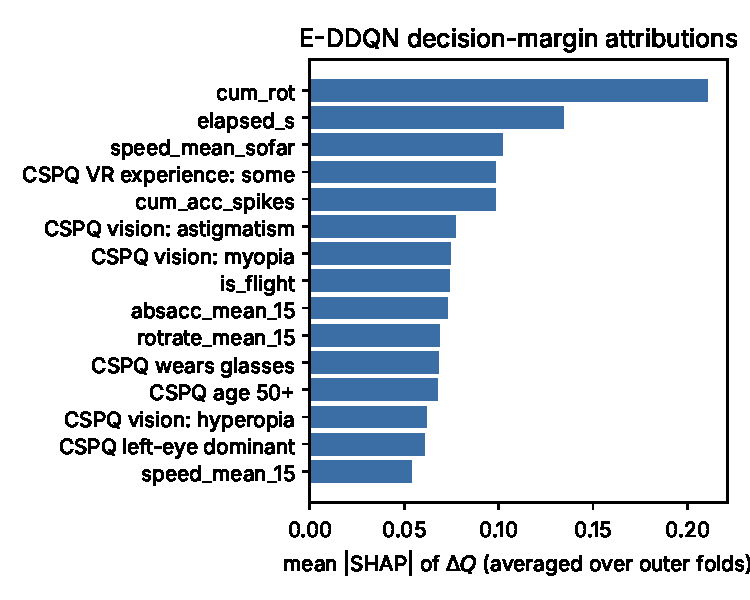
\includegraphics[width=0.92\columnwidth]{figs/shap_margin.pdf}
\caption{Mean absolute SHAP value of the E-DDQN decision margin $\Delta Q$, averaged over the five outer folds (one model per fold; attributions on that fold's test groups).}
\label{fig:shap}
\end{figure}
